\documentclass[10pt,a4paper, singlespace]{article}
\setlength\parindent{24pt}
\usepackage[utf8]{inputenc}
\usepackage{amsmath}
\usepackage{amsfonts}
\usepackage{hyperref}
%\usepackage{setspace}
\usepackage{amssymb}
\usepackage{graphicx}
\usepackage{caption}
\usepackage{subcaption}
%\usepackage{subfig}
\usepackage{minted}
\usepackage{float}
%\usepackage{minted}
\usepackage[top=1.25in, bottom=1.25in, left=1.5in, right=1.5in]{geometry}


\author{Michael Flossmann and Amanda Boström}
\title{Case Study - ROS on Raspberry Pi + Camera}
\date{\today}

\begin{document}
\maketitle

\begin{center}
  \emph{All code for this exercise can be found at \\ \url{https://github.com/maenhetten/finding-big-zebro}}
\end{center}

\section*{Introduction}

The following report recounts the work put into and results acquired from a motion detection node, running on a ROS system on the Raspberry Pi 2 Model B, using a Raspberry Pi Camera module.\\
The objective of the case study was to use image subtraction and filtering to obtain motion detection in the camera image, publishing on a topic whenever motion was detected. \\
The motion detection system was tested on zebrafish larvae in a lab setting, tracking their swimming patterns.



\section{Preparation}
\subsection{Hardware}

For this project, the Raspberry Pi 2 Model B was used. It runs on an ARM core and includes a camera interface, to which the Raspberry Pi Camera module was attached.

\subsection{Software Installation}

The first step of the project was to set up the Raspberry Pi, and installing an operating system on it. \\
At first, as specified in the assignment description, Ubuntu 14.04 was installed. When running Ubuntu, however, the camera did not respond. Due to this, after several attempts at solving the issue, Raspbian Jessie was installed instead. This is the operating system used for the rest of the project. \\
For using the camera module the RaspiCam library was used. The library provides the class RaspiCam that gives full control of the camera, and works well with the OpenCV library. \\
OpenCV is an open source library specifically made for use within computer vision applications. It provides methods for processing the images acquired through the camera. Among the methods used for the project were image subtraction, filtering, and contour finding methods. Exactly how the methods were incorporated into the ROS node are described in greater detail in the next section. \\
\subsection{Plan of action}
Before starting the implementation process of the motion detection system a plan of action was discussed. The objective of the project was considered and milestones were set accordingly. Future development was also discussed, which were to be implemented provided there was time left at the end of the project. In the plan of action, the focus was to make a system that was easy to use for the prospective user, and to, of course, have a functioning motion detection program.

\section{Implementation}


\subsection{Debug window}

In order to effectively oversee the results and to debug the project during development, the very first step was to implement a debug window. The debug window essentially shows a visualization of the image and motion data that the system is receiving and processing.\\
The debug window is also used to produce images showing the results of the project.\\
\subsection{Filtering}

For eliminating noise in the acquired image, a Gaussian filter, specifically the OpenCV-method GaussianBlur, was used.

\begin{figure}[H]
	\centering
	\begin{subfigure}[b]{0.5\textwidth}
		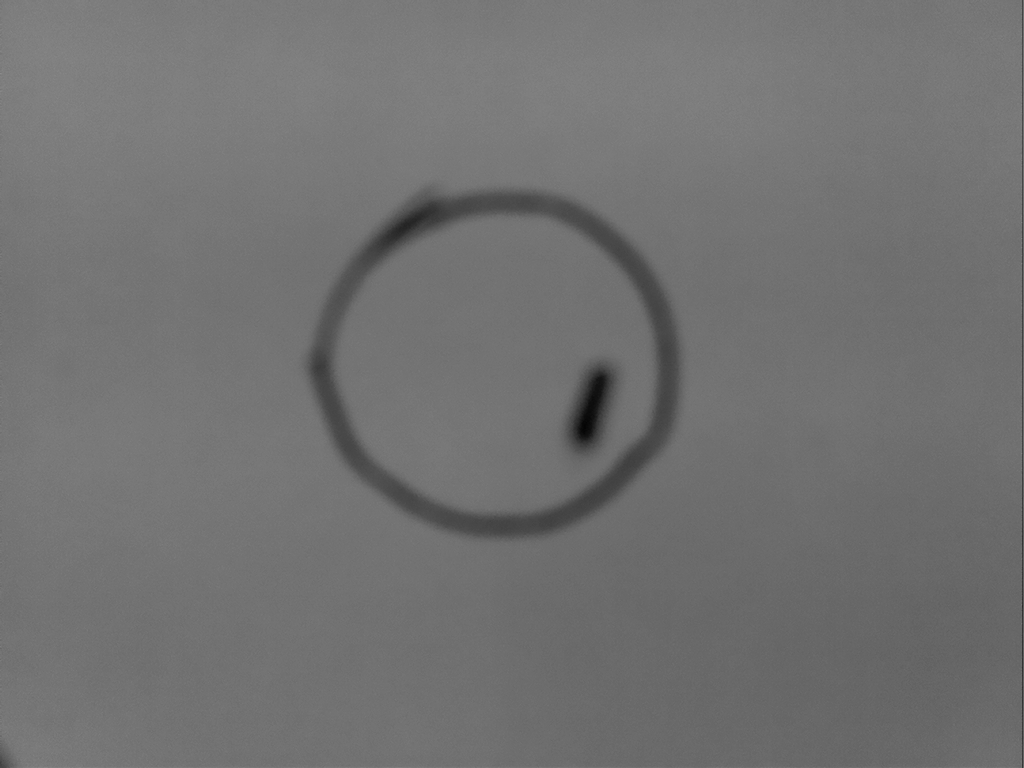
\includegraphics[width=0.8\textwidth]{without_filter.png}
		\caption{The unfiltered image.}
		\label{fig:unfiltered}
	\end{subfigure}\hfill
	\begin{subfigure}[b]{0.5\textwidth}	
		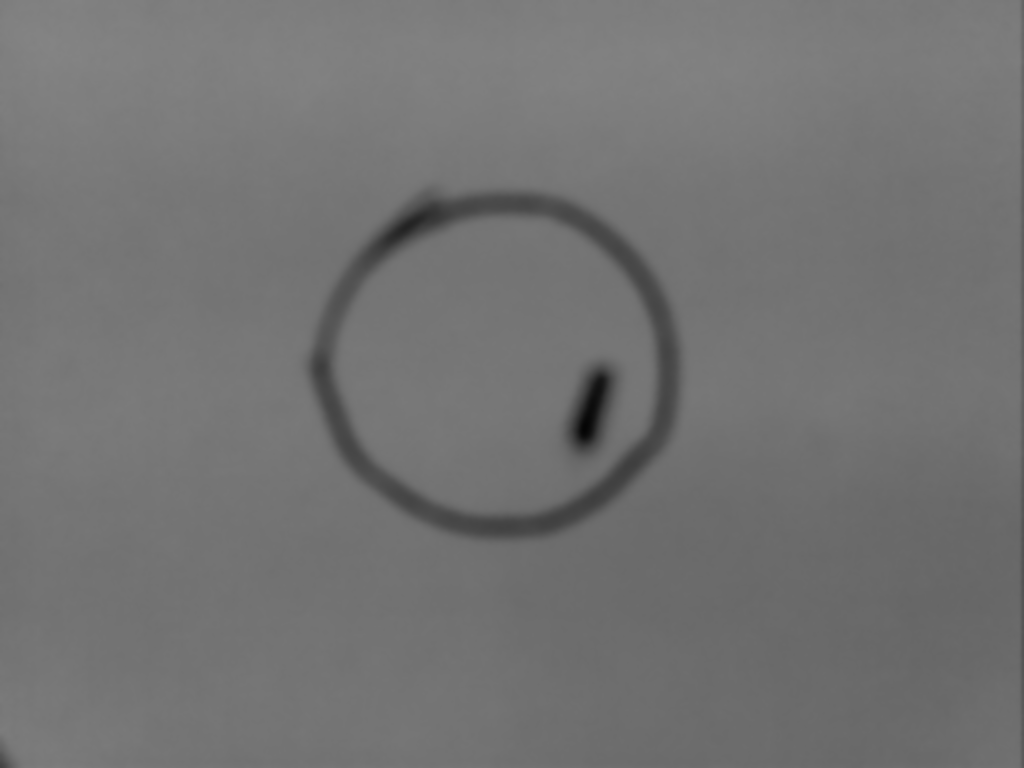
\includegraphics[width=0.8\textwidth]{gaussian_blur.png}
		\caption{Gaussian filter applied.}
		\label{fig:gaussian}
	\end{subfigure}\hfill
	\caption{Noise removal.}
	\label{fig:fitlering}
\end{figure} 

%\subsection*{Image subtraction}
\subsection{Thresholding}
In order to clearly distinguish between objects in the image, the OpenCV-method Threshold was used. Threshold takes a value and sets every pixel with a value below that to black and every pixel above it to white.\\
Thresholding the image is key for identifying moving objects, by removing irrelevant objects out of the image. The threshold value needs to be adjusted based on the object that is followed, and the lighting conditions for the camera, as this affects the pixel values in the image.\\ 

\begin{figure}[H]
	\centering
	\begin{subfigure}[b]{0.5\textwidth}
		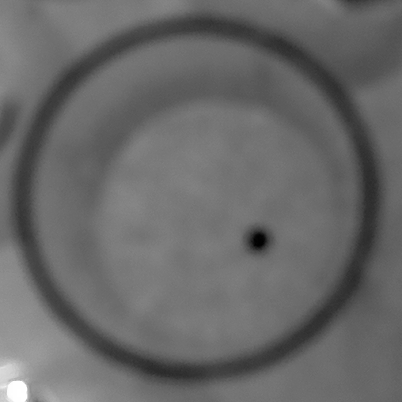
\includegraphics[width=0.8\textwidth]{image_raw.png}
		\caption{The raw image.}
		\label{fig:raw}
	\end{subfigure}\hfill
	\begin{subfigure}[b]{0.5\textwidth}	
		
\includegraphics[width=0.8\textwidth]{image_threshold.png}
		\caption{Image after thresholding.}
		\label{fig:threshold}
	\end{subfigure}\hfill
	\caption{Object detection.}
	\label{fig:thresholding}
\end{figure} 

\subsection{Identifying contours}
Using the OpenCV function findContours was central to detecting and following relevant obstacles, i.e. the zebrafish larvae. FindContours provides information about the object's location. The contours are displayed as pink dots in center points of the detected objects in the debug window.\\
Below, in figure \ref{fig:contours}, the results can be seen on some of the dummy objects that were used for testing the system before trying it out on the zebrafish themselves.\\

\begin{figure}[H]
	\centering
	\begin{subfigure}[b]{0.5\textwidth}
		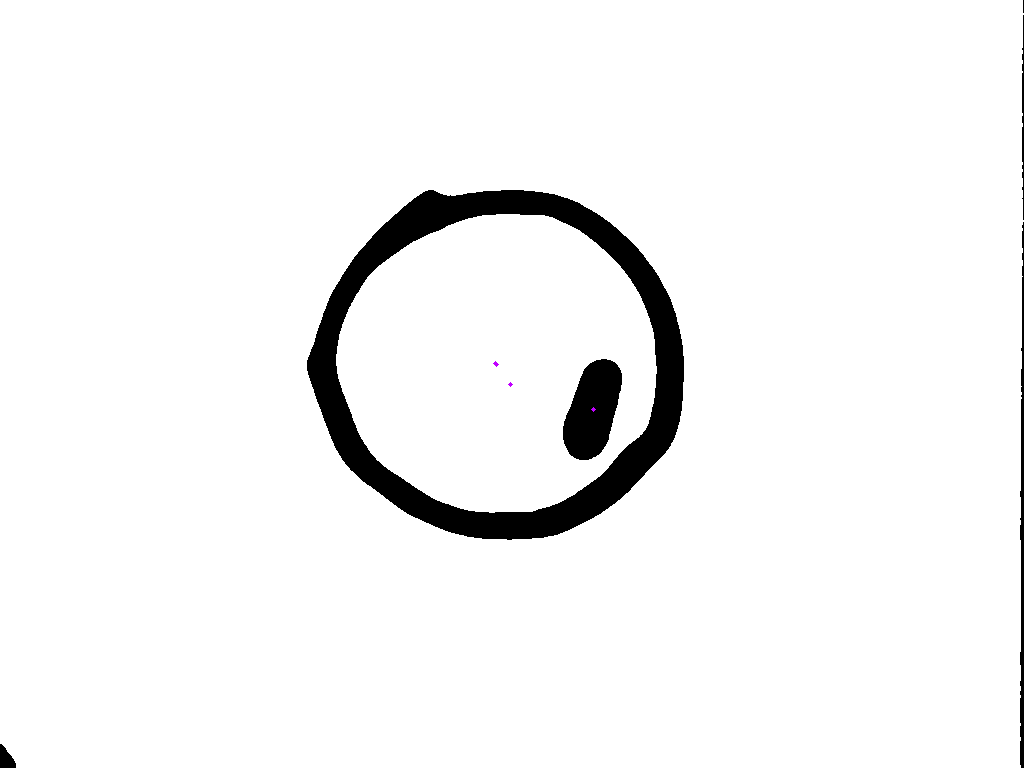
\includegraphics[width=0.8\textwidth]{contour_centers.png}
		%\caption{The unfiltered image.}
		\label{fig:unfiltered}
	\end{subfigure}\hfill
	\begin{subfigure}[b]{0.5\textwidth}	
		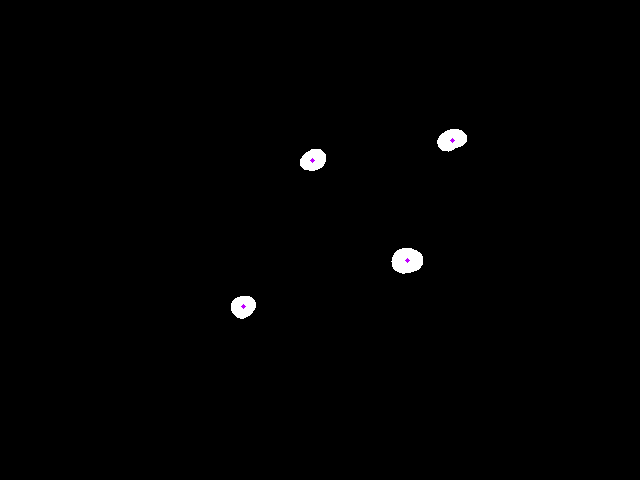
\includegraphics[width=0.8\textwidth]{contour_detection.png}
		%\caption{Gaussian filter applied.}
		\label{fig:gaussian}
	\end{subfigure}\hfill
	\caption{Contour identification.}
	\label{fig:contours}
\end{figure} 

\subsection{Placement indicator}
In order to ensure that the testing dish holding the larvae is placed in the correct location for detecting motion, a circle is drawn onto the debug window. The circle can be used for visually adjusting the test dish position. The result is shown below, in figure \ref{fig:placement}.\\

\begin{figure}[H]
	\centering	
	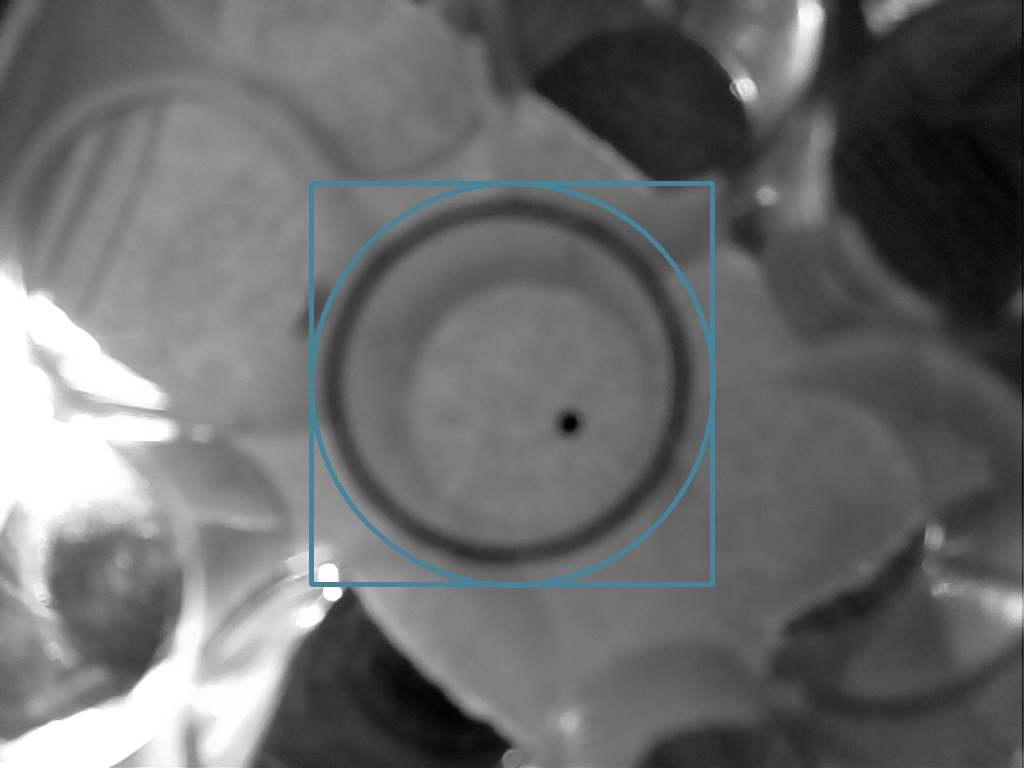
\includegraphics[width=0.8\textwidth]{placement_circle.png}
	\caption{Placement circle.}
	\label{fig:placement}
\end{figure} 

\subsection{Dynamic reconfiguration}
For facilitating usage of the system for a user without programming knowledge, a dynamic reconfiguration window was implemented. The window enables reconfiguration of relevant variables, during runtime, for adapting the system to the current environment and the individual fish larvae. Lighting and size of the larvae among other aspects affect the required settings. All of these can be visually adjusted by using the debug window. Some aspects of the image processing can also be turned on or off.\\
The variables that are currently dynamically reconfigurable are as follows, including type:\\
\\
1. thresholding limit (integer)\\
2. relative square size (double; size of placement circle)\\
3. gaussian blur (boolean)\\
4. threshold (boolean)\\
5. find contours (boolean)\\
6. gaussian filter kernel (integer)\\
7. gaussian filter sigma (integer)\\
8. minimum specimen size (integer; relative to square size)\\
9. minimum specimen size (integer; relative to square size) \\

\section{Testing with live specimen}
The objective of the case study was to develop a motion detection system, that could track the swimming patterns of zebrafish larvae. The zebrafish larvae that were used for the study were about 96 hours old, and around 2mm in length. At this age, the larvae are mostly pigmented around the eyes, becoming increasingly transparent towards the tail. Below, in figure \ref{fig:zebro}, a magnified image of a zebrafish is shown.\\

\begin{figure}[H]
	\centering	
	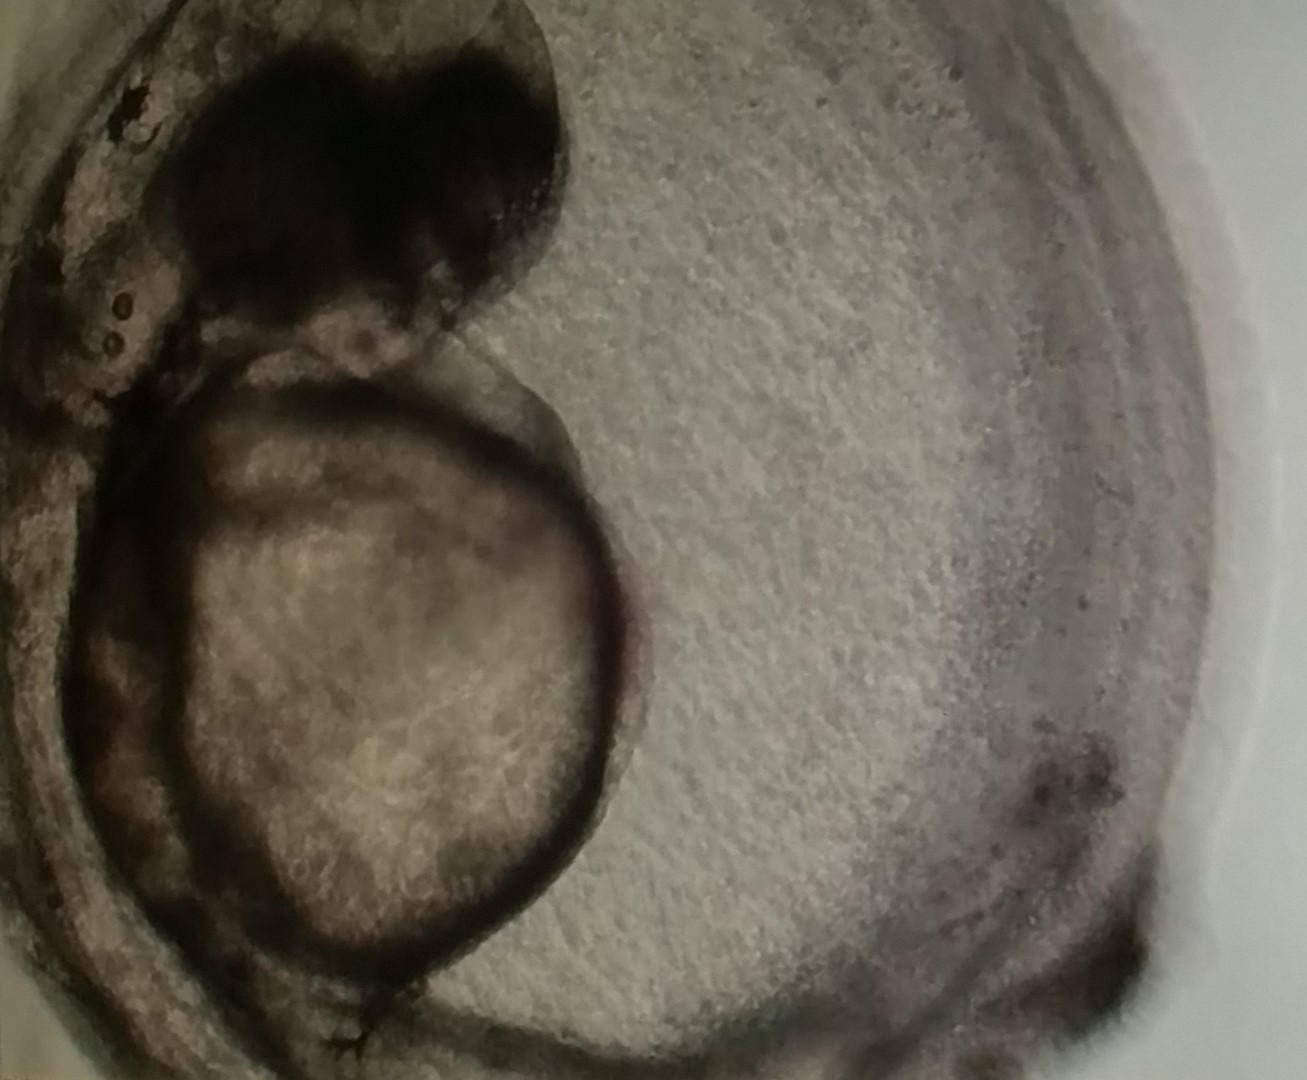
\includegraphics[width=0.6\textwidth]{zebro.jpg}
	\caption{The zebrafish larva.}
	\label{fig:zebro}
\end{figure}

\subsection{The setup}
The motion detection system was tested in a lab environment, using a petri dish, and  placing a single larvae in it, along with some water for it to swim in. The Raspberry Pi and the camera module were suspended above the petri dish. For optimal placement, the debug window and the placement circle were utilized. The final setup is shown below, in figure \ref{fig:setup}.

\begin{figure}[H]
	\centering	
	\includegraphics[width=0.5\textwidth]{awesome.jpg}
	\caption{The setup at the biology lab.}
	\label{fig:setup}
\end{figure} 

\subsection{The results}
The single larvae was detected by the system, and was able to track its movements, publishing its position at every iteration in the terminal window. Below are some sample images from the testing, showcasing the results.\\

\begin{figure}[H]
	\centering
	\begin{subfigure}[b]{0.3\textwidth}
		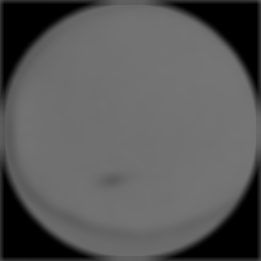
\includegraphics[width=0.8\textwidth]{fish_raw.png}
		\caption{The raw image.}
		\label{fig:depth-b}
	\end{subfigure}\hfill
	\begin{subfigure}[b]{0.3\textwidth}	
		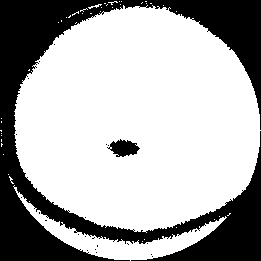
\includegraphics[width=0.8\textwidth]{fish_threshold_unblurred.png}
		\caption{The thresholded image.}
		\label{fig:depth-b-no-nan}
	\end{subfigure}\hfill
	\begin{subfigure}[b]{0.3\textwidth}
	\includegraphics[width=0.8\textwidth]{ fish_detection.png}
		\caption{The detected fish.}
		\label{fig:depth-bilateral-no-nan}
	\end{subfigure}\hfill
	\caption{The zebrafish larvae.}
	\label{fig:testing}
\end{figure} 

\section{Future development}
Some issues are left unsolved for the project, in order to deploy it as an actual research tool for a typical laboratory environment. Given more time these could be solved and the tool further developed for user friendliness.\\ 
Among these is the issue of the larvae blending in with the borders of the placement circle when swimming too close to them. This makes the system consider it a part of the circle. This could be solved by background subtraction. Specifically, storing one background image if the algorithm found the specimen and removing the place where the specimen was found in the background image.\\
Another issue left to solve is that the positions recorded need to be connected to a timestamp, in order to calculate the speeds of the larvae, which is a relevant piece of information for the biologist researching the zebrafish.   



\end{document}